\documentclass{article}
\usepackage{amsmath}
%\usepackage{psfig}

\usepackage{amsmath}
\usepackage{graphicx}
\usepackage{float}
\usepackage{amssymb} 
\usepackage{amsthm}
\usepackage{pgf}
\usepackage{tikz}
\usetikzlibrary{automata,shapes.multipart} %
\usetikzlibrary{arrows,petri}
\usepackage[latin1]{inputenc}
%\usepackage[noend]{algorithmic}
\usepackage{algorithm}
%\usepackage{algo}
\usepackage{epsfig}
\usepackage{subfigure}
\usepackage{multirow}
\usepackage{url}


\title{Cosmos User Manual}
\author{Beno\^it Barbot}

\begin{document}
\maketitle


This is the user manual for the tool Cosmos version 1.

\section{File Format}
\subsection{Generalized Stochastic Petri Net (.gspn)}
This file format is used to describe GSPN.
First we describe an example:\\
\begin{figure}[h]
  \centering
  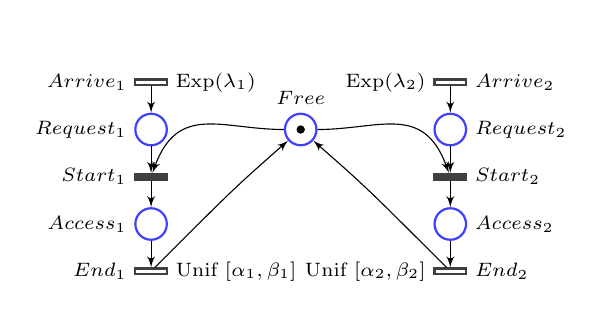
\begin{tikzpicture}[node distance=0.6cm,>=stealth',auto]
{\scriptsize
  \tikzstyle{place}=[circle,thick,draw=blue!75,minimum size=4mm]
  \tikzstyle{transition}=[rectangle,thick,draw=black!75,
  minimum width=4mm,inner sep=0pt,minimum height=.7mm]

    \node [] (i1)       {};
    \node [transition,label=left:$Arrive_1$,label=right:Exp($\lambda_1$)] (tr1) [below of =i1]{};
    \node [place,label=left:$Request_1$] (r1) [below of=tr1]  {};
    \node [transition,,label=left:$Start_1$,fill=black!75] (ta1) [below of =r1]{}; %label=right:$(\mbox{pri}_1\colon w_1)$
    \node [place,label=left:$Access_1$] (a1)  [below of=ta1] {};
    \node [transition,label=left:$End_1$,label=right:{\hspace{-0mm}{\scriptsize Unif $[\alpha_1,\beta_1]$}}] (ti1) [below of =a1]{};
    \node [place,tokens=1,label=above:$Free$] (f) [right of=r1,xshift=13mm]    {};
    \node [place,label=right:$Request_2$] (r2) [right of=f,xshift=13mm]    {};
   \node [transition,label=right:$Arrive_2$,label=left:Exp($\lambda_2$)] (tr2) [above of =r2]{};
    \node [] (i2) [above of=tr2]    {};
    \node [transition,label=right:$Start_2$,fill=black!75] (ta2) [below of =r2]{}; %label=left:$(\mbox{pri}_2\colon w_2)$,
    \node [place,label=right:$Access_2$] (a2) [below of=ta2]    {};
    \node [transition,label=right:$End_2$,label=left:{\hspace{-2mm}{\scriptsize Unif $[\alpha_2,\beta_2]$}}] (ti2) [below of =a2]{};
%\draw [-latex'] (i1) to (tr1);
\draw [-latex'] (tr1) to (r1);
\draw [-latex'] (r1) to (ta1);
\draw [-latex'] (ta1) to (a1);
\draw [-latex'] (a1) to (ti1);
%\draw [-latex'] (i2) to (tr2);
\draw [-latex'] (tr2) to (r2);
\draw [-latex'] (r2) to (ta2);
\draw [-latex'] (ta2) to (a2);
\draw [-latex'] (a2) to (ti2);
\draw [-latex'] (f) .. controls +(0:10mm) and +(110:10mm) .. (ta2);
\draw [-latex'] (f) .. controls +(180:10mm) and +(70:10mm) .. (ta1);
\draw [-latex'] (ti1) .. controls +(45:15mm)  .. (f); %and +(260:20mm)
\draw [-latex'] (ti2) .. controls +(135:15mm) .. (f); %and +(280:20mm) 
}
\end{tikzpicture} 
  \caption{Infinite-state GSPN  model of a shared memory system.}
  \label{fig:sharedmem}
  % \vspace*{-.3cm}
\end{figure}
This GSPN is described by the following text:
\begin{verbatim}
const double lambda1 = 1;
const double lambda2 = 2;
const double alpha1 = 1;
const double alpha2 = 1;
const double beta1 = 5;
const double beta2 = 5;

NbPlaces = 5;
NbTransitions = 6;

PlacesList = { 
   Request_1, Request_2,
   Access_1, Access_2,
   Free
} ;

TransitionsList = { 
   Arrive_1,Arrive_2,
   Start_1 ,Start_2,
   End_1   ,End_2
} ;

Marking={
   (Request_1 , 0); (Request_2 , 0) ; 
   (Access_1 , 0) ; (Access_2 , 0) ;
   (Free, 1);
};

Transitions={
   (Arrive_1,EXPONENTIAL(lambda1),1,1, SINGLE); 
   (Arrive_2,EXPONENTIAL(lambda2),1,1, SINGLE);
   (Start_1,DETERMINISTIC(0),1,1); 
   (Start_2,DETERMINISTIC(0),1,1);
   (End_1,UNIFORM(alpha1,beta1),1,1); 
   (End_2,UNIFORM(alpha2,beta2),1,1);
};

InArcs={
   (Request_1,Start_1,1); (Free,Start_1,1);
   (Request_2,Start_2,1); (Free,Start_2,1);
   (Access_1,End_1,1);
   (Access_2,End_2,1);
};

OutArcs={
   (Arrive_1,Request_1,1); 
   (Arrive_2,Request_2,1);
   (End_1,Free,1);
   (End_2,Free,1);
};
\end{verbatim}

{\bf Description:}
The first bloc is a list of constants definition, constants can be
either \verb|double| or \verb|int|.\\
Then we specify the number of place and transitions with:
\verb|NbPlaces = 5; NbTransitions = 6;|\\
The list of place name and transition name is given in the
\verb|PlacesList| and \verb|TransitionsList| statement.\\
The initial marking of the net is given as a set of pairs
in the \verb|Marking| statement.\\
The transition distribution is given as a set of tuples like
this one:\\ \verb|(Arrive_1,EXPONENTIAL(lambda1),1,1, SINGLE)|
each tuple contain first the name of the transition then
the probability distribution with some parameters, then two positive
reals define the priority and weight of the event generated.
For exponential distribution we can specify the policy of service
which can be \verb|SINGLE,INFINITE,MULTIPLE(n)|.\\
Finally come the description of arcs of the net with the 
\verb|InArcs|,\verb|OutArcs| and \verb|InhibitorsArcs| statements.



\subsubsection{Grammar}
the complete grammar is:
\begin{verbatim}
$accept: GSPN "end of file"

GSPN: declarations definitions
    | declarations definitions redifinitions

declarations: Constants Sizes Lists
            | Sizes Lists

Constants: Constant
         | Constant Constants

Constant: 'const' 'int' str '=' IntStringFormula ';'
        | 'const' 'double' str '=' RealStringFormula ';'

IntStringFormula: ival
                | str
                | '(' IntStringFormula ')'
                | IntStringFormula '+' IntStringFormula
                | IntStringFormula '-' IntStringFormula
                | IntStringFormula '*' IntStringFormula
                | IntStringFormula '^' IntStringFormula
                | FLOOR '(' IntStringFormula ')'
                | FLOOR '(' IntStringFormula '/' IntStringFormula ')'
                | MIN '(' IntStringFormula ',' IntStringFormula ')'
                | MAX '(' IntStringFormula ',' IntStringFormula ')'

RealStringFormula: rval
                 | ival
                 | str
                 | '(' RealStringFormula ')'
                 | RealStringFormula '/' RealStringFormula
                 | RealStringFormula '+' RealStringFormula
                 | RealStringFormula '-' RealStringFormula
                 | RealStringFormula '*' RealStringFormula
                 | RealStringFormula '^' RealStringFormula
                 | FLOOR '(' RealStringFormula ')'
                 | MIN '(' RealStringFormula ',' RealStringFormula ')'
                 | MAX '(' RealStringFormula ',' RealStringFormula ')'

Sizes: NbPlaces NbTransitions
     | NbTransitions NbPlaces

NbPlaces: 'NbPlaces' '=' ival ';'
        | 'NbPlaces' '=' str ';'

NbTransitions: 'NbTransitions' '=' ival ';'
             | 'NbTransitions' '=' str ';'

Lists: PlacesList TransitionsList
     | TransitionsList PlacesList

PlacesList: 'PlacesList' '=' '{' PLabels '}' ';'

PLabels: str
       | PLabels ',' str

TransitionsList: 'TransitionList' '=' '{' TLabels '}' ';'

TLabels: str
       | TLabels ',' str

definitions: PlacesDef TransitionsDef InArcs OutArcs
           | PlacesDef TransitionsDef InArcs OutArcs Inhibitors

PlacesDef: 'Marking' '=' '{' PLACES '}' ';'

PLACES: PLACE
      | PLACES PLACE

PLACE: '(' str ',' IntStringFormula ')' ';'

TransitionsDef: 'Transition' '=' '{' TRANSITIONS '}' ';'

TRANSITIONS: TRANSITION
           | TRANSITIONS TRANSITION

TRANSITION: '(' str ',' dist ',' PRIORITY ',' WEIGHT ')' ';'
          | '(' str ',' 'EXPONENTIAL' '(' RealStringFormula ')' ',' PRIORITY ',' 
            WEIGHT ',' SERVICE ')' ';'
          | '(' str ',' IMDT ',' PRIORITY ',' WEIGHT ')' ';'

dist: str '(' params ')'

params: RealStringFormula
      | params ',' RealStringFormula

WEIGHT: RealStringFormula

PRIORITY: RealStringFormula

SERVICE: 'SINGLE'
       | 'INFINITE'
       | 'MULTIPLE' '(' ival ')'
       | 'MULTIPLE' '(' str ')'

InArcs: 'InArcs' '=' '{' incells '}' ';'

incells: incell
       | incells incell

incell: '(' str ',' str ',' IntStringFormula ')' ';'
      | '(' str ',' str ')' ';'

OutArcs: 'OutArcs' '=' '{' outcells '}' ';'

outcells: outcell
        | outcells outcell

outcell: '(' str ',' str ',' IntStringFormula ')' ';'
       | '(' str ',' str ')' ';'

Inhibitors: 'inhibitor' '=' '{' inhibcells '}' ';'

inhibcells: inhibcell
          | inhibcells inhibcell

inhibcell: '(' str ',' str ',' IntStringFormula ')' ';'
         | '(' str ',' str ')' ';'
\end{verbatim}




\end{document}
